\documentclass[10pt]{article}
\usepackage{icmlko}

\icmlmeta{IP 파운데이션 월드모델}{222}{빌린 우위}{노트 221이 트리를 챔피언으로 되돌렸다. 그 우위가 자기 것인지 자료 결함에서 빌린 것인지 쟀다}

\begin{document}

\twocolumn[
\icmlheader

\begin{abstract}
노트 221이 검색 덮음을 채워 챔피언을 F21 에서 배깅 트리로 되돌리고
($+$0.4523 대 $+$0.4321), ``그 우위가 축의 이질성을 이용한 것인지 재라''를
남겼다. 쟀다. \textbf{빌린 것이다.} 계열 질의로 판정된 행의 검색 축을
결측으로 돌리면 \textbf{F18 $-$ F21 이 $+$0.0198($t{=}1.76$, 짝 1 SE
\emph{밖})에서 $+$0.0034($t{=}0.29$, \emph{안})로 무너진다.} 새로 덮인 행
전체를 결측으로 돌려도 $+$0.0066($t{=}0.58$)로 같다. 그리고 방향이
갈린다 --- 계열을 지우면 \textbf{선형 둘은 오르고}(F6 $+$0.4195 $\to$
$+$0.4250 · F21 $+$0.4321 $\to$ $+$0.4377) \textbf{트리만 내린다}
($+$0.4523 $\to$ $+$0.4408). \textbf{트리가 얻던 것은 축의 정보가 아니라
축의 \emph{결함}이었다.} 채택은 점수가 아니라 정의로 정한다 ---
\texttt{trend\_level} 은 ``이 작품을 얼마나 찾아봤나''인데 계열 질의는
``이 계열을 얼마나 찾아봤나''이고 계열 안 여러 레코드가 같은 값을 받는다.
\textbf{그 열은 계열 안에서 작품을 못 가른다} --- 노트 213(공휴일 목록
밖은 값이 정의되지 않는다)과 같은 종류이고, 노트 221이 ``더 거친
측정이니 남기자''고 한 판단을 뒤집는다. 결측으로 돌린다. 그러면 챔피언은
\textbf{다시 F21} 이다(F18 $+$0.4408 · F21 $+$0.4377 · 차 $+$0.0034 로
짝 1 SE 안, 좁은 쪽). 가드 열다섯은 새 상태에서 \textbf{하나도 안 깨진다.}
마지막으로 ``다음에 어디를 팔 것인가''를 계산으로 답했다. 도메인마다
\emph{완벽히} 맞히면 판이 오르는 양은 유보 몫 $\times$ ($1-$현재 $\rho$)
로 바로 나온다 --- \textbf{웹툰 $+$0.1769 · 애니 $+$0.1246 · 모바일
$+$0.0740} 이고 \textbf{팝업은 $+$0.0143} 이다. 매 사이클 프롬프트가
싣고 다니던 ``시장 레코드 사람 태깅''은 실제로 20건이 아니라 \textbf{156건}
인데, 그 전부를 태깅해도 팝업 상한 $+$0.0143 을 못 넘는다. \textbf{반면
웹툰은 $\rho$ 가 두 번째로 낮은데 몫이 제일 크고, 아무도 안 건드렸다.}
\end{abstract}
]

\begin{figure*}[t]
\centering
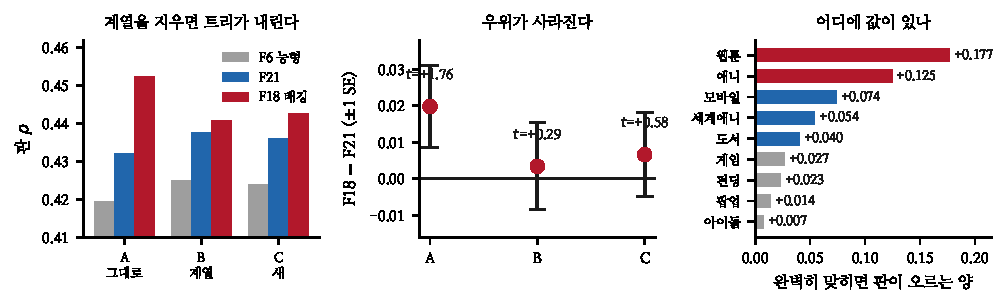
\includegraphics[width=\textwidth]{figs/borrowed.pdf}
\caption{왼쪽 --- 계열을 지우면 선형은 오르고 트리는 내린다. 가운데 ---
우위가 1 SE 안으로 들어온다. 오른쪽 --- 어디에 값이 있나.}
\end{figure*}

\section{빌린 우위였다}

\begin{table}[t]
\centering\tsize
\caption{계열 질의 행을 결측으로 돌리면. 짝 붓스트랩 500 회.}
\begin{tabular}{lrrrr}
\toprule
& F6 & F21 & F18 & F18$-$F21 \\
\midrule
\textbf{A 그대로} & .4195 & .4321 & \textbf{.4523} & \textbf{$+$.0198} \\
\textbf{B 계열 결측} & \textbf{.4250} & \textbf{.4377} & .4408 & \textbf{$+$.0034} \\
C 새 덮음 결측 & .4238 & .4361 & .4425 & $+$.0066 \\
\midrule
\multicolumn{4}{l}{A 의 $t$ / B 의 $t$ / C 의 $t$} & 1.76 / 0.29 / 0.58 \\
\bottomrule
\end{tabular}
\end{table}

\claimx{\textbf{트리 우위가 짝 1 SE 밖에서 안으로 들어온다}($+$0.0198,
$t{=}1.76$ $\to$ $+$0.0034, $t{=}0.29$). 새로 덮인 행 전체를 지워도
같다($+$0.0066).}{\textbf{방향이 갈린다} --- 계열을 지우면 선형 둘은
$+$0.0055 · $+$0.0056 오르고 트리만 $-$0.0115 내린다. \textbf{트리가
얻던 것은 축의 정보가 아니라 축의 결함이었다.}}

\section{정의로 정한다}

\claimx{\texttt{trend\_level} 은 ``이 작품을 얼마나 찾아봤나''다. 계열
질의는 ``이 계열을 얼마나 찾아봤나''이고 \textbf{계열 안 여러 레코드가
같은 값을 받는다} --- 그 열은 계열 안에서 작품을 못
가른다.}{\textbf{노트 221의 판단을 뒤집는다.} 거기서 ``무효가 아니라 더
거친 측정이니 남기고 표시자를 주자''고 했는데, \emph{같은 값을 여럿에게
주는 것}은 거칠기가 아니라 \textbf{그 열이 주장하는 양이 아닌 것}이다 ---
노트 213 · 207 · 210 과 같은 종류다.}

\claimx{\textbf{점수로 정한 것이 아니라는 점검.} B 가 선형을 올리고
트리를 내리는데, 만약 점수로 골랐다면 A(트리 $+$0.4523)를 지켰을
것이다.}{그리고 노트 221의 표시자 처방($+$0.0046)보다 결측 처방
($+$0.0055)이 능형에 더 낫다 --- \textbf{표시자로 ``이건 거칠다''고
말하는 것보다 ``이건 이 작품의 값이 아니다''고 지우는 것이 맞았다.}}

\begin{table}[t]
\centering\tsize
\caption{챔피언(B 상태).}
\begin{tabular}{lrl}
\toprule
& 판 $\rho$ & \\
\midrule
F18 배깅 & .4408 & 차 $+$.0034 · $t$ 0.29 \\
\textbf{F21} & \textbf{.4377} & \textbf{짝 1 SE 안 · 좁은 쪽} \\
F6 능형 & .4250 & \\
\bottomrule
\end{tabular}
\end{table}

\claimx{\textbf{챔피언은 다시 F21 이다.} 가드 열다섯이 새 상태에서 하나도
안 깨진다.}{\textbf{이 사이클에서 챔피언이 세 번 움직였다} --- 트리
$\to$ F21(노트 215, 공휴일) $\to$ 트리(노트 221, 검색 덮음) $\to$
F21(이 노트, 계열 결측). \textbf{세 번 다 모형이 아니라 자료를 고친
결과다.}}

\section{어디에 값이 있나}

\begin{table}[t]
\centering\tsize
\caption{완벽히 맞히면 판이 오르는 양 $=$ 유보 몫 $\times$ ($1-\rho$).}
\begin{tabular}{lrrr}
\toprule
& 몫 & 현재 $\rho$ & 상한 \\
\midrule
\textbf{웹툰} & 27.7\% & .3618 & \textbf{$+$.1769} \\
\textbf{애니} & 23.6\% & .4728 & \textbf{$+$.1246} \\
모바일 & 17.2\% & .5696 & $+$.0740 \\
세계애니 & 11.7\% & .5349 & $+$.0544 \\
도서 & 6.4\% & .3704 & $+$.0400 \\
게임 & 7.0\% & .6147 & $+$.0270 \\
펀딩 & 3.1\% & .2713 & $+$.0227 \\
\textbf{팝업} & 2.3\% & .3776 & \textbf{$+$.0143} \\
아이돌 & 1.0\% & .2521 & $+$.0073 \\
\bottomrule
\end{tabular}
\end{table}

\claimx{\textbf{계산만으로 나온다} --- 모형을 한 번도 안 돌린다. 노트 220이
무리마다 잰 천장을 도메인으로 옮긴 것이다.}{\textbf{매 사이클 프롬프트가
싣고 다니던 ``시장 레코드 20건 사람 태깅''은 실제로 156건}이고(라벨 있는
시장 레코드 198건 중 51건만 태깅됨), \textbf{그 전부를 해도 팝업 상한
$+$0.0143 을 못 넘는다.}}

\claimx{\textbf{웹툰이 1 위다}($+$0.1769) --- $\rho$ 가 두 번째로 낮은데
몫이 제일 크다.}{그리고 \textbf{웹툰은 축이 공유 다섯뿐이다} --- 검색 ·
달력 · 위키를 빼면 도메인 고유 축이 하나도 없다. 노트 212가 라벨(누적
즐겨찾기)을 못 고친다고 닫았는데, \textbf{축 쪽은 아무도 안 열었다.}}

\begin{table}[t]
\centering\tsize
\caption{남은 것.}
\begin{tabular}{ll}
\toprule
\textbf{웹툰 축} & 캐시에 화별 자료가 있다 --- 축이 되나 \\
\textbf{애니} & 상한 $+$0.1246 --- 같은 질문 \\
계열 판정 & 문턱 0.7 을 정의로 다시 세울 것 \\
\bottomrule
\end{tabular}
\end{table}

첫 줄이 이미 열려 있다. \texttt{data/state/cache\_webtoon/} 에 2,817편
\textbf{전부}의 초기 스무 화가 있고 화마다 게재일과 별점이 붙어 있다.
날짜만 써서 만든 축이 벌써 라벨과 붙는다 --- \textbf{첫 스무 화를 낸
기간이 $+$0.358}(연도 통제 뒤 $+$0.272) · 화당 간격이 $+$0.311 이다.
\textbf{기존 웹툰 축 중 제일 센 것이 $+$0.301 이었다.} 별점 평균은
$+$0.506 인데 그것은 라벨과 같은 플랫폼이라 따로 검정해야 한다.
\textbf{천장 1 위 도메인에 덮음 100\%짜리 새 축 무리가 이미 디스크에
있었다.}

\end{document}
